\documentclass[14pt,a4paper]{article}
\setlength\parindent{0pt}
\setlength{\parskip}{1em}
\usepackage{array}
\usepackage{amsmath}
\usepackage{amsfonts}
\usepackage{amssymb}
\usepackage{mathrsfs}
\usepackage{graphicx}
\usepackage[margin=1.0in]{geometry}
%\usepackage[toc,page]{appendix}

\begin{document}
\title{Generalizing Complex/Hyper-complex Convolutions to Vector Map Convolutions}
\author{Chase J Gaudet \\  cjg7182@louisiana.edu
   \and Anthony S Maida \\  maida@louisiana.edu}
\maketitle

\begin{abstract}
The core reasons that complex and hyper-complex valued neural networks offer improvements over their real-valued counterparts is the weight sharing mechanism and treating the dimensions of multidimensional data as a single entity.
Here we introduce vector map convolutions which capture both of these properties provided by complex/hyper-complex convolutions, while dropping the unnatural dimensionality constraints they impose.
This is achieved by introducing a learned parameter that combines the dimensions instead of the  complex algebra, such as the Hamilton product for quaternions.
\end{abstract}

\section{Introduction}
While the large majority of work in the area of machine learning (ML) has been done using real-valued models, recently there has been an increase in use of complex and hyper-complex models.
These models have been shown to handle multidimensional data more effectively and require fewer parameters than their real-valued counterparts.

For tasks with two dimensional input vectors, complex-valued neural networks (CVNNs) are a natural choice.
For example in audio signal processing the magnitude and phase of the signal can be encoded as a complex number.
Since CVNNs treat the magnitude and phase as a single entity a single activation captures their relationship as opposed to real-valued networks.
CVNNs have been shown to outperform or match real-valued networks, while sometimes at a lower parameter count \cite{trabelsi+al-2018-complexconv, aizenberg2018image}.
However, most real world data has more than two dimensions such as color channels of images or anything in the realm of 3D space.

The quaternions number system extends the complex numbers.
These hyper-complex numbers are composed of one real and three imaginary components making them ideal for three or four dimensional data.
Quaternion neural networks (QNNs) have enjoyed a surge in recent research and show promising results \cite{takahashi2017remarks, bayro2018geometric, Gaudet2018, parcollet2017deep, parcollet2017quaternion, parcollet2018quaternion-A, parcollet2018quaternion-B, parcollet2019quaternion}.
Quaternion networks have been shown to be very effective at capturing the relationship of multidimensional data of four or fewer dimensions.
For example the red, green, and blue color channels of images for image processing networks needs to capture the cross channel relationships of these colors as they contain important information to support good generalization \cite{kusamichi2004new, isokawa2003quaternion}.
Real-valued networks treat the color channels as independent entities unlike quaternion networks.
Parcollet et al. \cite{parcollet2019quaternion} showed that a real-valued encoder-decoder fails to reconstruct unseen color images due to it failing to capture local (color) and global (edges and shapes) features independently, while the quaternion encoder-decoder is able to do so.
Their conclusion is that the Hamilton product of the quaternion algebra allows the quaternion network to encode the color relation since it treats the colors as a single entity.
Another example is 3D spatial coordinates for robotic and human-pose estimation.
Pavllo et al. \cite{pavllo2018quaternet} showed improvement on short-term prediction on the Human3.6M dataset using a network that encoded rotations as quaternions over Euler angles.

We suggest that the main reason that these complex networks to outperform real-valued networks is their underlying algebra which treats the multidimensional data as a single entity.
This allows the complex networks to capture the relationships between the dimensions without trade off of learning global features.
However, using complex or hyper-complex numbers limits the dimensions to either two for complex or four with quaternions.
There are higher dimension hyper-complex such as octonions at eight dimensions, but they are a non-associative algebra.
Therefore, the present paper proposes: 1) to create a system that mimics the concepts of complex and hyper-complex numbers for neural networks, which is treating multidimensional input as a single entity and weight sharing, but is not constrained to certain dimensions\footnote{The full code is available at https://github.com/gaudetcj/VectorMapConv}; 2) to increase their local learning capacity by introducing a learnable parameter inside the multidimensional dot product. 
Our experiments herein show that these novel vector map convolutions seem to capture all the benefits of complex and hyper-complex networks, while improving their ability to capture internal latent relations, and avoiding the dimensionality restriction.


\section{Motivation for Vector Map Convolutions}
Most data used in ML is multidimensional and, to achieve good performance models, must both capture the local relations within the input features \cite{tokuda2003trajectory, matsui2004quaternion}, as well as global features, for example edges or shapes composed by a group of pixels.
Complex and hyper-complex models have been shown to be able to both capture these local relations better than real-valued models, but also to do so at a reduced parameter count due to their weight sharing property.
However, these models are constrained to two or four dimensions.
Below we detail the work done showing how hyper-complex models capture these local features as well as the motivation to generalize them to any number of dimensions.

Consider the most common form of representing an image, which is by using three 2D matrices where each matrix corresponds to a color channel.
Traditional real-valued networks treat this input as a group of unidimensional elements that may be related to one another, but not only does it need to try to learn that relation, it also needs to try to learn global features such as edges and shapes.
By encoding the color channels into a quaternion each pixel is treated as a whole entity strongly related to one another.
It has been shown that the quaternion algebra is responsible for allowing QNNs to capture these local relations. 
For example, Parcollet et al. \cite{parcollet2019quaternion} showed that a real-valued encoder-decoder fails to reconstruct unseen color images due to it failing to capture local (color) and global (edges and shapes) features independently, while the quaternion encoder-decoder is able to do so.
Their conclusion is that the Hamilton product of the quaternion algebra allows the quaternion network to encode the color relation since it treats the colors as a single entity.
The Hamilton product forces a different linear combination of the internal elements to create each output element.
This is seen in Fig.~\ref{f:hamilton} from \cite{parcollet2018quaternion-A}, which shows how a real-valued model looks converted to a quaternion model.
Notice that the real-valued model treats local and global weights at the same level, while the quaternion model learns these local relations during the Hamilton product.
The weight sharing property can also be seen where each element of the weight is used four times, reducing the parameter count by a factor of four from the real-valued model.

\begin{figure}
	\centering
		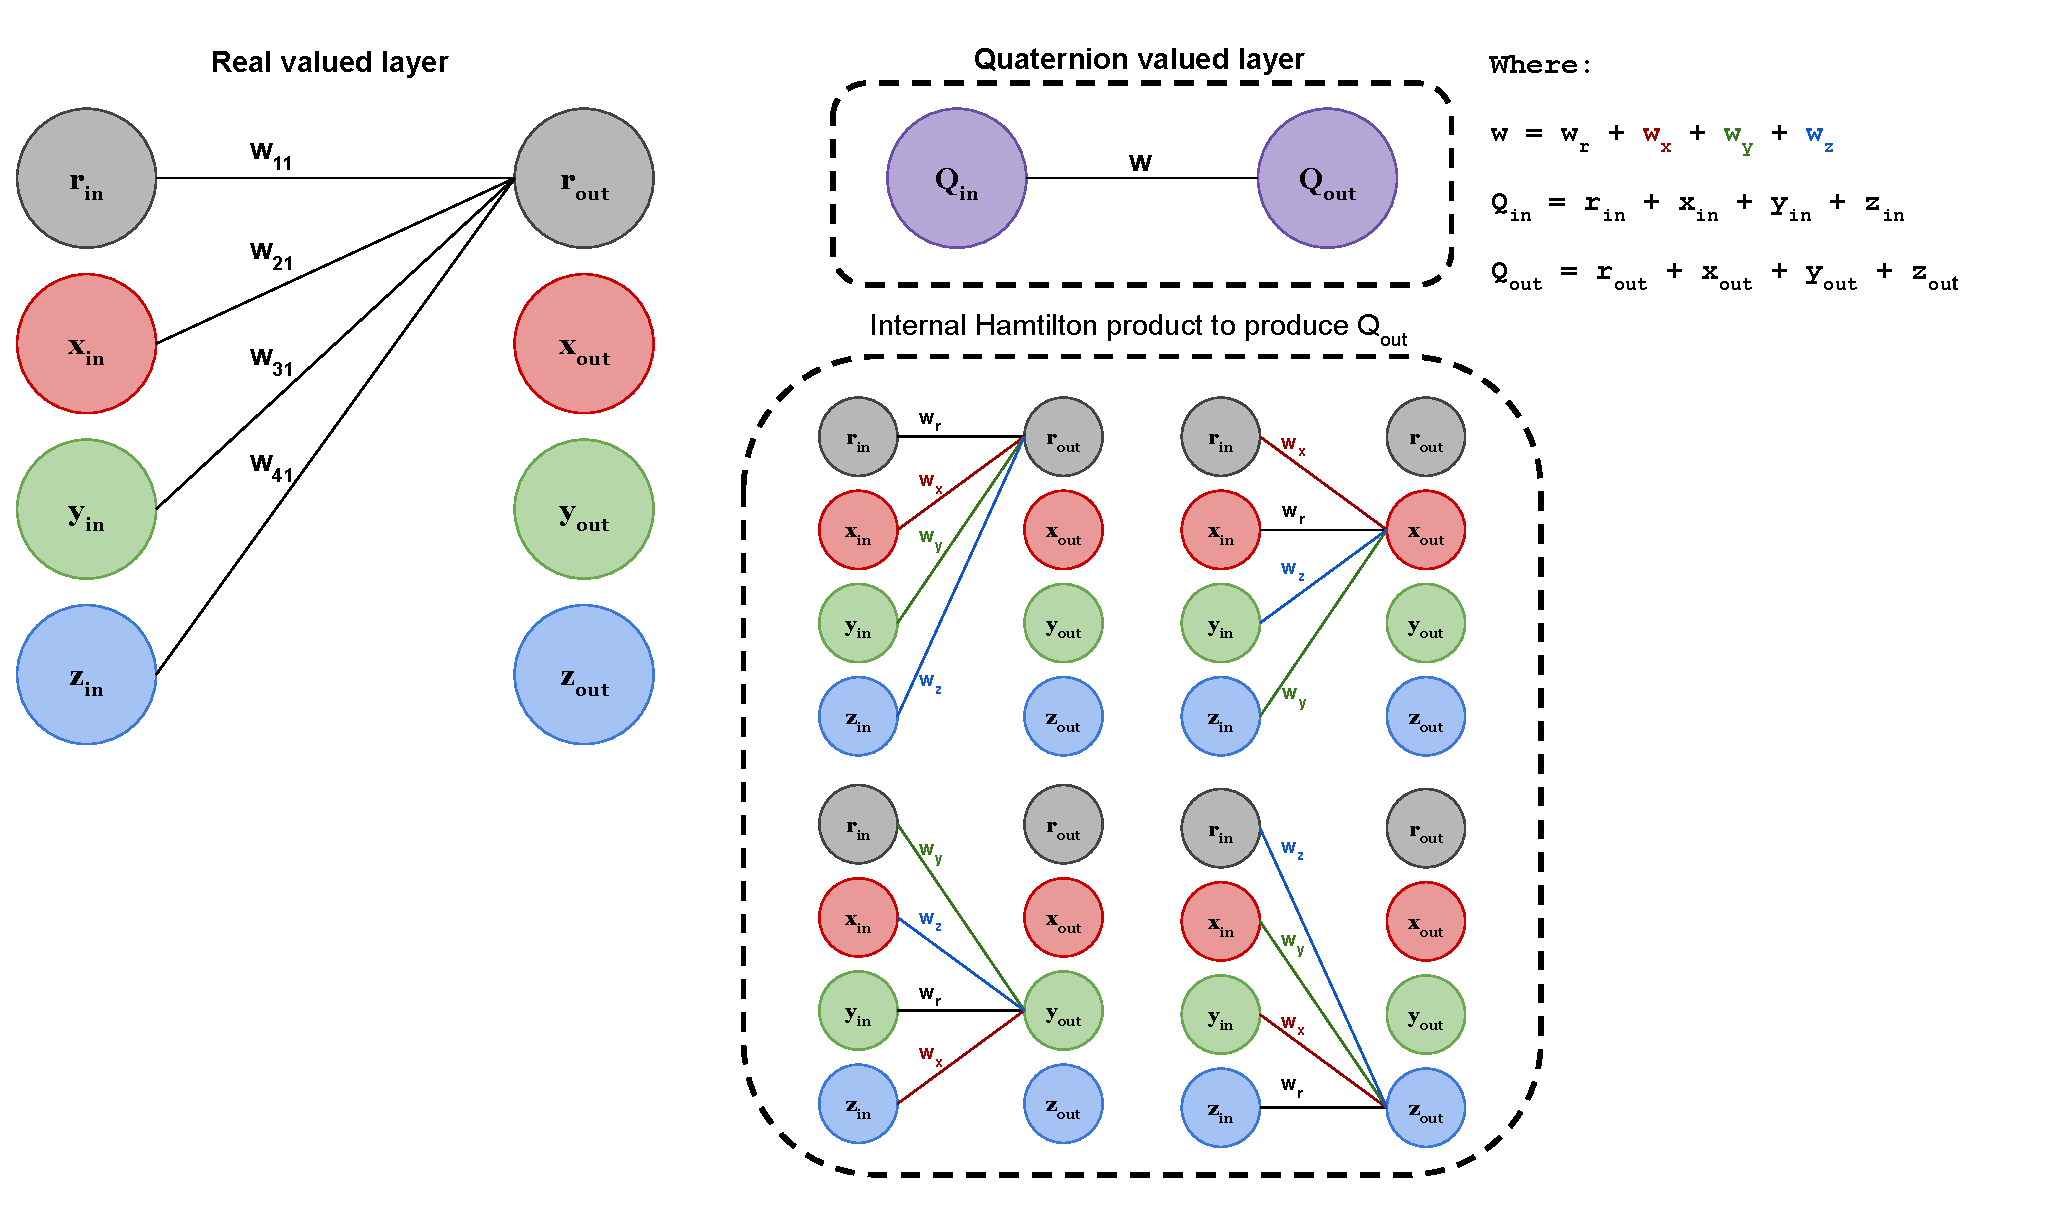
\includegraphics[width=1.0\columnwidth]{figures/RealToQuaternion.pdf}
		\caption{Illustration of the difference between a real-valued layer (left) and quaternion-valued layer (right). The quaternion's Hamilton product shows the internal relation learning ability not present in the real-valued.}
	\label{f:hamilton}
\end{figure}

The advantages of hyper-complex networks on multidimensional data seems clear, but what about niche cases where there are higher dimensions than four?
Examples include applications where one needs to ingest extra channels of information on top of RGB for image processing, like satellite images which have several bands.
To overcome this limitation we introduce vector map convolutions, which attempt to generalize the benefits of hyper-complex networks to any number of dimensions.
We also add a learnable set of parameters that modify the linear combination of internal elements.


\section{Vector Map Components}
This section will include the work done to obtain a working vector map network.
This includes the vector map convolution operation and the weight initialization used.

\subsection{Vector Map Convolution}
Vector map convolutions use a similar convolution to that of complex \cite{trabelsi+al-2018-complexconv} and quaternion \cite{Gaudet2018} convolutions but in a more general way that does not bind it to a hyper-complex algebra.
In both complex and quaternion convolution the input to the convolution layer and the kernels of the convolution layer both have multiple axes, two for complex (real and imaginary) and four for quaternion (real and three imaginary: i, j, k).
They also both produce feature maps of the same number of axes, which can be thought of as feature vectors (vector of feature maps).
The quaternion convolution operation for can be seen in Fig.~\ref{f:quatconv}.
One can see that each axis of the resultant feature vector is actually a linear combination of a different input axis convolved against a different kernel axis.
This also causes these convolution operations to have a sort of weight sharing and makes them have a lower parameter count versus a real-valued network with the same number of convolution kernels.

\begin{figure}
	\centering
		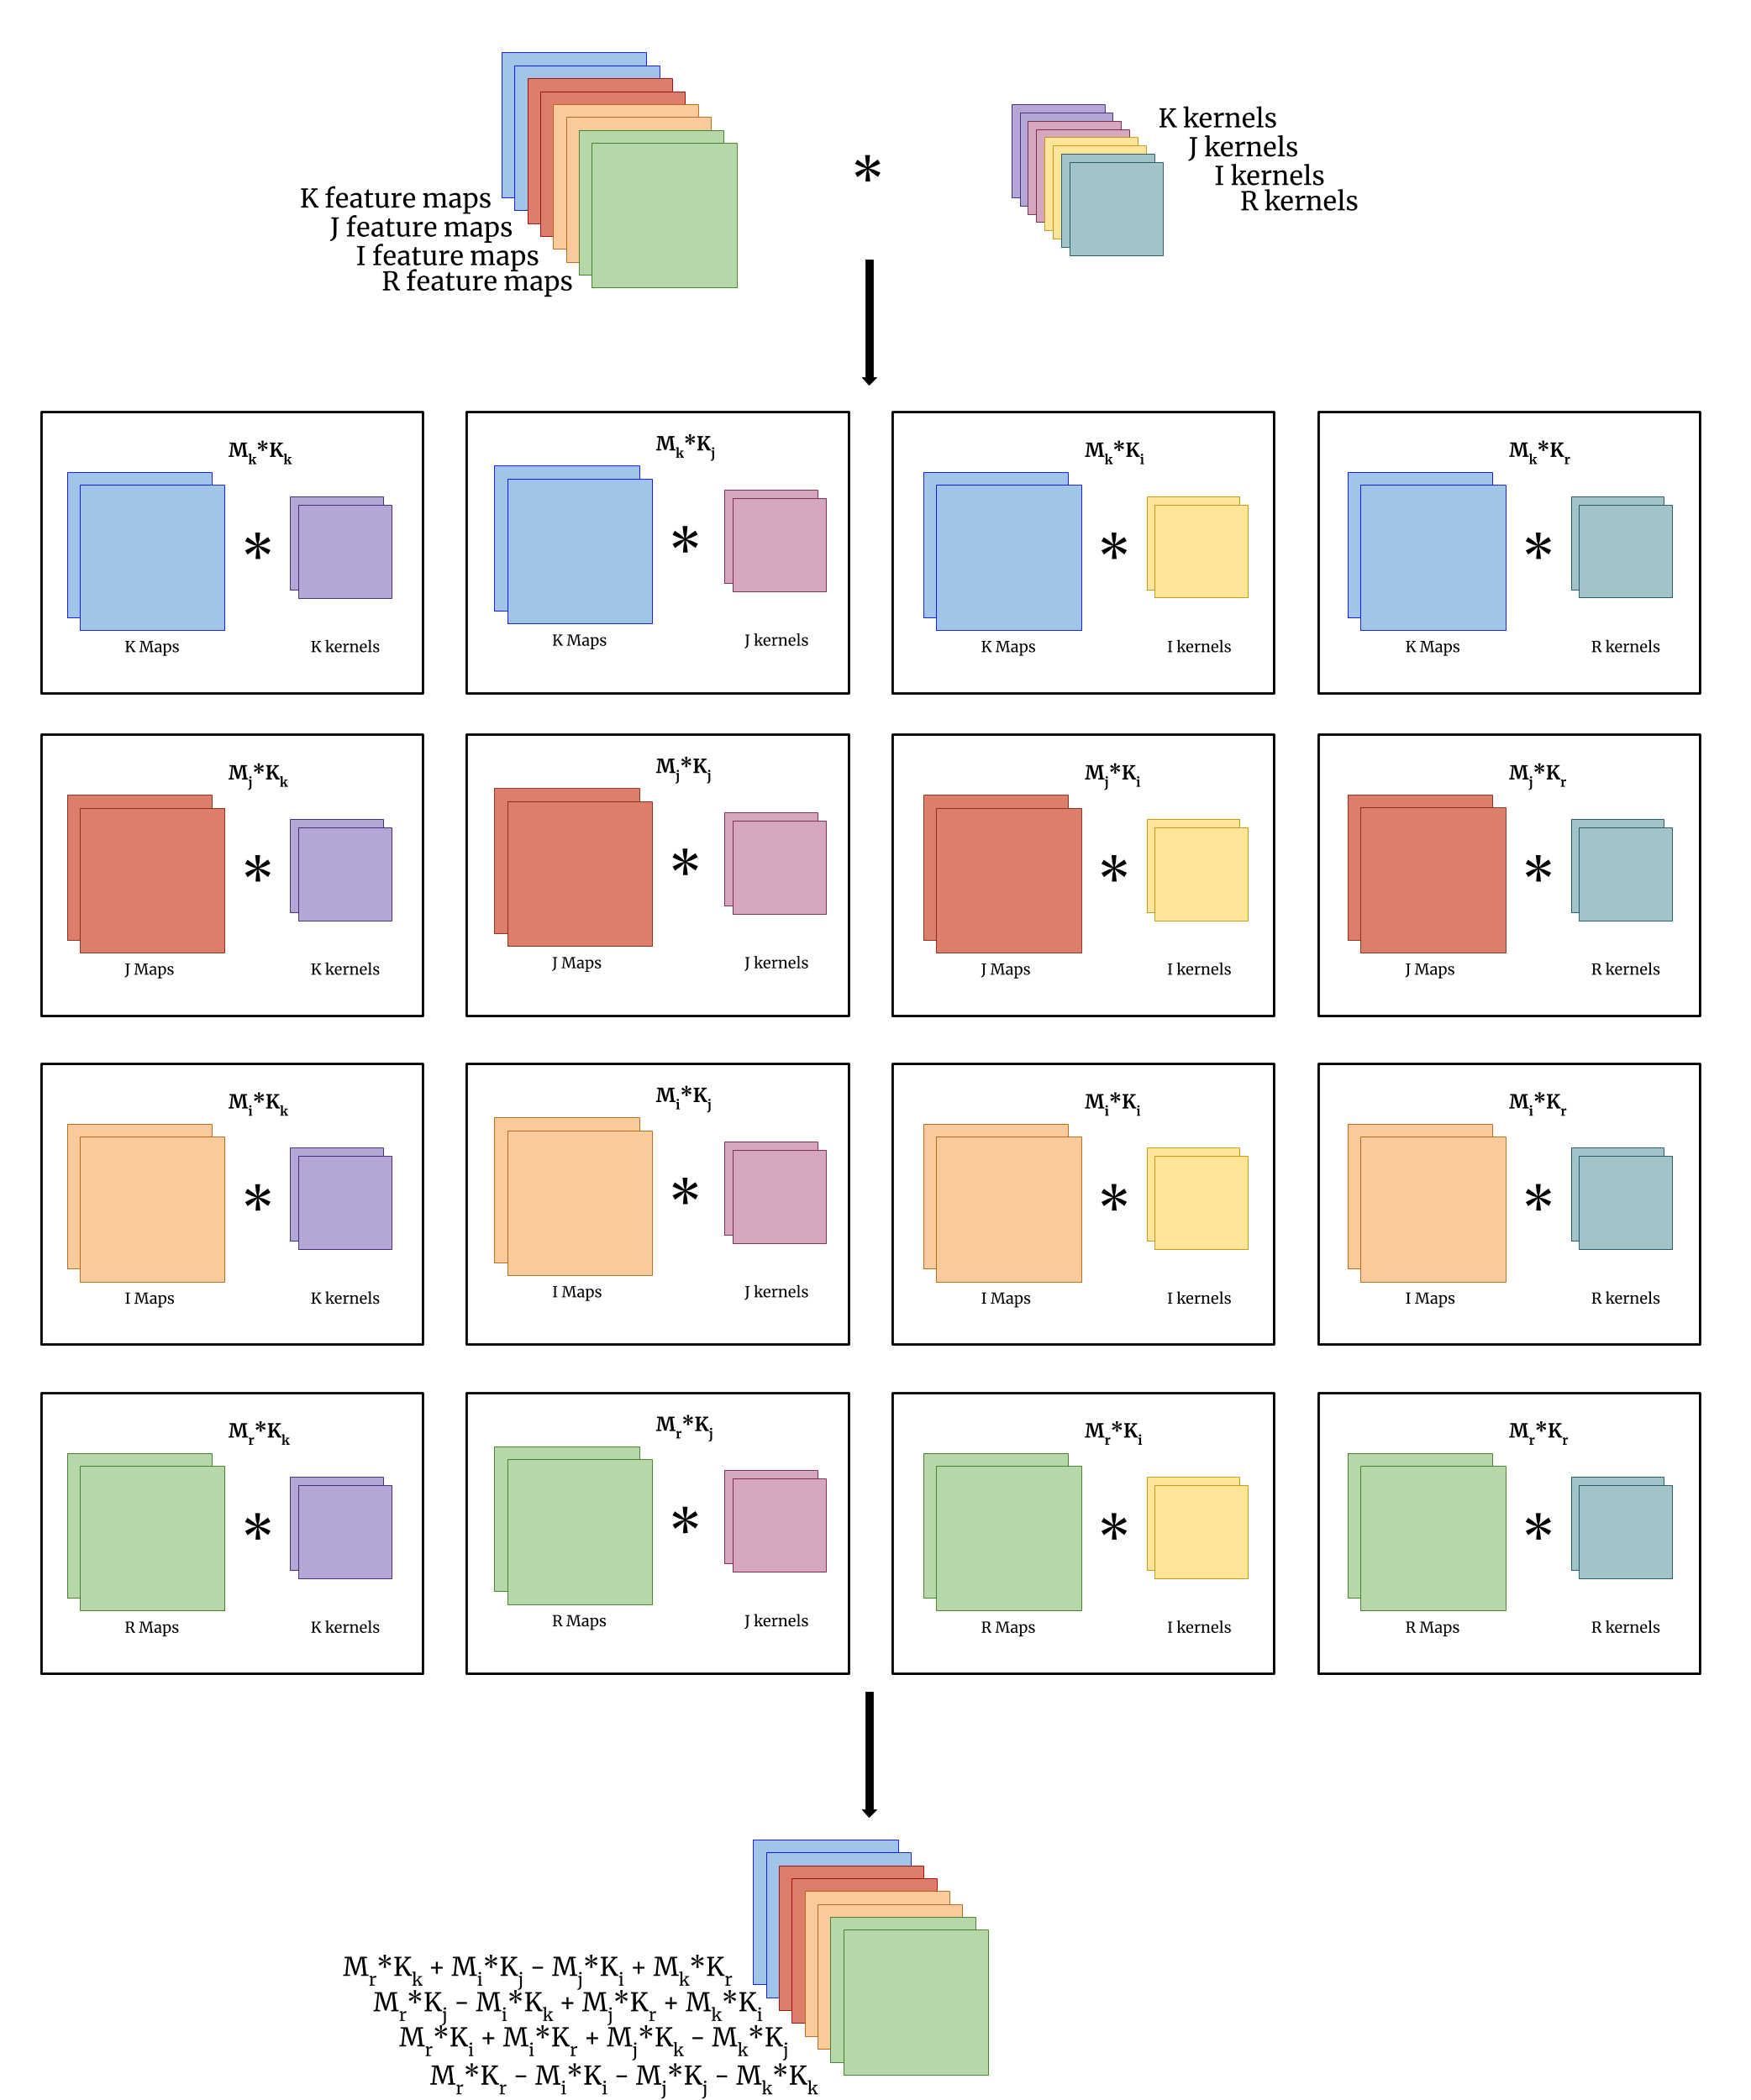
\includegraphics[width=1.0\columnwidth]{figures/quatconv.png}
		\caption{An illustration of quaternion convolution.}
	\label{f:quatconv}
\end{figure}

Building on the idea of linearly combining feature maps, vector map convolutions can take a user defined number of axes $D_\mathrm{vm}$.
That is, $D_\mathrm{vm}$ is not constrained to have values 2, 4, or 8 corresponding to the hyper-complex numbers.
The axes are permuted one to the right for each axis beyond the first to obtain the rows of the convolution matrix.
Also instead of a linear combination a learned weight is used instead.
This weight is defined as a matrix $\textbf{L} \in \mathbb{R}^{D_\mathrm{vm}\times D_\mathrm{vm}}$.
As an example let us look at quaternion convolution in matrix form and then the vector map convolution with four axes in matrix form.
The result of convolving a quaternion filter matrix $\textbf{W}=\textbf{A}+\textit{i}\textbf{B}+\textit{j}\textbf{C}+\textit{k}\textbf{D}$ by a quaternion vector $\textbf{h}=\textbf{w}+\textit{i}\textbf{x}+\textit{j}\textbf{y}+\textit{k}\textbf{z}$ is another quaternion,
\begin{equation}
\begin{bmatrix}
 \mathscr{R}(\textbf{W}\ast \textbf{h}) \\ 
 \mathscr{I}(\textbf{W}\ast \textbf{h}) \\
 \mathscr{J}(\textbf{W}\ast \textbf{h}) \\
 \mathscr{K}(\textbf{W}\ast \textbf{h}) 
\end{bmatrix}
=
\begin{bmatrix}
 \textbf{A} & -\textbf{B} & -\textbf{C} & -\textbf{D} \\
 \textbf{B} & \textbf{A} & -\textbf{D} & \textbf{C} \\
 \textbf{C} & \textbf{D} & \textbf{A} & -\textbf{B} \\
 \textbf{D} & -\textbf{C} & \textbf{B} & \textbf{A} \\
\end{bmatrix}
\ast
\begin{bmatrix}
 \textbf{w} \\ 
 \textbf{x} \\
 \textbf{y} \\
 \textbf{z}
\end{bmatrix} ,
\label{e:quatconv}
\end{equation}

\noindent
where $\mathbf{A}$, $\mathbf{B}$, $\mathbf{C}$, and $\mathbf{D}$ are real-valued matrices and 
$\mathbf{w}$, $\mathbf{x}$, $\mathbf{y}$, and $\mathbf{z}$ are real-valued vectors.
More explanation is given in \cite{Gaudet2018}.

The vector map convolution with $D_\mathrm{vm} = 4$ and $\textbf{L}$ is a $4\times4$ real matrix, is given by
\begin{equation}
\begin{bmatrix}
 \mathscr{R}(\textbf{W}\ast \textbf{h}) \\ 
 \mathscr{I}(\textbf{W}\ast \textbf{h}) \\
 \mathscr{J}(\textbf{W}\ast \textbf{h}) \\
 \mathscr{K}(\textbf{W}\ast \textbf{h}) 
\end{bmatrix}
=
%\begin{bmatrix}
%\textbf{A}\textbf{L$_{1,1}$} & \textbf{B}\textbf{L$_{1,2}$} & \textbf{C}\textbf{L$_{1,3}$} & \textbf{D}\textbf{L$_{1,4}$} \\
%\textbf{D}\textbf{L$_{2,1}$} & \textbf{A}\textbf{L$_{2,2}$} & \textbf{B}\textbf{L$_{2,3}$} & \textbf{C}\textbf{L$_{2,4}$} \\
%\textbf{C}\textbf{L$_{3,1}$} & \textbf{D}\textbf{L$_{3,2}$} & \textbf{A}\textbf{L$_{3,3}$} & \textbf{B}\textbf{L$_{3,4}$} \\
%\textbf{B}\textbf{L$_{4,1}$} & \textbf{D}\textbf{L$_{4,2}$} & \textbf{C}\textbf{L$_{4,3}$} & \textbf{A}\textbf{L$_{4,4}$} \\
%\end{bmatrix}
%\begin{bmatrix}
% L_{1,1}\cdot \textbf{A} & L_{1,2}\cdot\textbf{B} & L_{1,3}\cdot\textbf{C} & L_{1,4}\cdot\textbf{D} \\
% L_{2,1}\cdot \textbf{D} & L_{2,2}\cdot\textbf{A} & L_{2,3}\cdot\textbf{B} & L_{2,4}\cdot\textbf{C} \\
% L_{3,1}\cdot \textbf{C} & L_{2,3}\cdot\textbf{D} & L_{3,3}\cdot\textbf{A} & L_{3,4}\cdot\textbf{B} \\
% L_{4,1}\cdot \textbf{B} & L_{2,4}\cdot\textbf{D} & L_{4,3}\cdot\textbf{C} & L_{4,4}\cdot\textbf{A} \\
%\end{bmatrix}
\mathbf{L}\odot
\begin{bmatrix}
 \textbf{A} & \textbf{B} & \textbf{C} & \textbf{D} \\
 \textbf{D} & \textbf{A} & \textbf{B} & \textbf{C} \\
 \textbf{C} & \textbf{D} & \textbf{A} & \textbf{B} \\
 \textbf{B} & \textbf{C} & \textbf{D} & \textbf{A} \\
\end{bmatrix}
\ast
\begin{bmatrix}
 \textbf{w} \\ 
 \textbf{x} \\
 \textbf{y} \\
 \textbf{z}
\end{bmatrix} .
\label{e:vmapconv}
\end{equation}

\noindent
The operator ``$\odot$'' is element-wise multiply.
Whereas the coefficients of the matrices that form $\mathbf{W}$ are fixed to $\pm1$ according to the quaternion algebra,
the sixteen parameters within $\mathbf{L}$ are unconstrained and intended to be learnable.
Thus, the vector map convolution is a generalization of complex, quaternion, or octonion convolution as the case may be,
but it also drops the constraints imposed by the associated hyper-complex algebra.

The question arises whether the empirical improvements observed in the use of complex and quaternion deep networks are best explained by the full structure of the hyper-complex algebra, or whether the weight sharing underlying the generalized
convolution is responsible for the improvement.

\subsection{Vector Map Weight Initialization}
Properly initializing of the weights has been shown to be vital to convergence of deep networks.
The weight initialization for vector map networks uses the same procedure seen in both deep complex networks \cite{trabelsi+al-2018-complexconv} and deep quaternion networks \cite{Gaudet2018}.
In both cases, the expected value of $|W|^2$ is needed to calculate the variance:
\begin{equation}
\mathbb{E}[|W|^2] = \int_{-\infty}^\infty x^2 f(x) ~dx
\label{e:expected}
\end{equation}
where $f(x)$ is a multidimensional independent normal distribution where the number of degrees of freedom is two for complex and four for hyper-complex.
Solving Eq.~\ref{e:expected} gives $2\sigma^2$ for complex and $4\sigma^2$ for quaternions.
Indeed, when solving Eq.~\ref{e:expected} for a multidimensional independent normal distribution where the number of degrees of freedom is $D_\mathrm{vm}$, the solution will equal $D_\mathrm{vm}\sigma^2$.
Therefore, in order to respect the Glorot and Bengio \cite{glorot2010understanding} criteria, the variance would be equal to :
\begin{equation}
\sigma = \sqrt{\frac{2}{D_\mathrm{vm}(n_{in} + n_{out})}}
\label{e:vmap-glorot}
\end{equation}
and in order to respect the He \cite{he2015delving} criteria, the variance would be equal to:
\begin{equation}
\sigma = \sqrt{\frac{2}{D_\mathrm{vm}n_{in}}}.
\label{e:vmap-he}
\end{equation}
This is used alongside a vector of dimension $D_\mathrm{vm}$ that is generated following a uniform distribution in the interval $[0, 1]$ and then normalized. The linear combination parameter $\textbf{L}$ in Eq.~\ref{e:vmapconv} is simply generated by randomly selecting from the set  $\{-1, 1\}$.


\section{Methods}
Our experiments cover simple image classification using CIFAR-10 and CIFAR-100 datasets \cite{krizhevsky2009learning}.
The CIFAR datasets are $32\times32$ color images of 10 and 100 classes respectively.
Each image contains only one class and labels are provided.
Since the CIFAR images are RGB, we use $D_\mathrm{vm} = 3$ for all the experiments.

For the architecture we use different Residual Networks taken directly from the original paper \cite{he2015deep}.
We ran direct comparison between real-valued, quaternion, and vector map networks on three different sizes: ReNet18, ResNet34, and ResNet50.
The only changes from the real-valued to vector map networks is the number of filters at each layer is changed such that the parameter count is roughly the same as the real-valued network.
Also for the vector map networks $\textbf{L}$ was initialized by randomly sampling a Bernoulli distribution with $p=1/2$ for each element and setting it to 1 if the distribution returned 1 or setting it to -1 if the distribution returned 0.
This was chosen as it matches closest to a complex or hyper-complex initialization.


\section{Experimental Results}
The results are shown in Table~\ref{t:results} as well as the validation loss and accuracy plots shown in Fig.~\ref{f:loss}. 
Also shown in Fig.~\ref{f:hist} is the histogram of $\textbf{L}$ for the ResNet18 vector map convolution network.
Notice how they appear to be normally distributed around the initial values of either -1 or 1.
We also include some visualizations of feature vector maps from the first convolution channel randomly selected on a few images in Fig.~\ref{f:samples}

\begin{table}[h]
	\centering
		\begin{tabular}{l c c c c}
			\hline
			Architecture & Params & CIFAR-10 & CIFAR-100 \\
			\hline
			ResNet18 Real & ??? & 5.92 & ??? \\
			ResNet18 Vector Map & ??? & 6.05 & ??? \\
			\hline
			ResNet34 Real & ??? & 5.73 & ??? \\
			ResNet34 Vector Map & ??? & 5.55 & ??? \\
			\hline
			ResNet50 Real & ??? & 6.10 & ??? \\
			ResNet50 Vector Map & ??? & 5.72 & ??? \\
			\hline
		\end{tabular}
	\caption{Percent error for classification on CIFAR-10 and CIFAR-100. Params is the total number of parameters.}
	\label{t:results}
\end{table}

\begin{figure}[h]
	\centering
		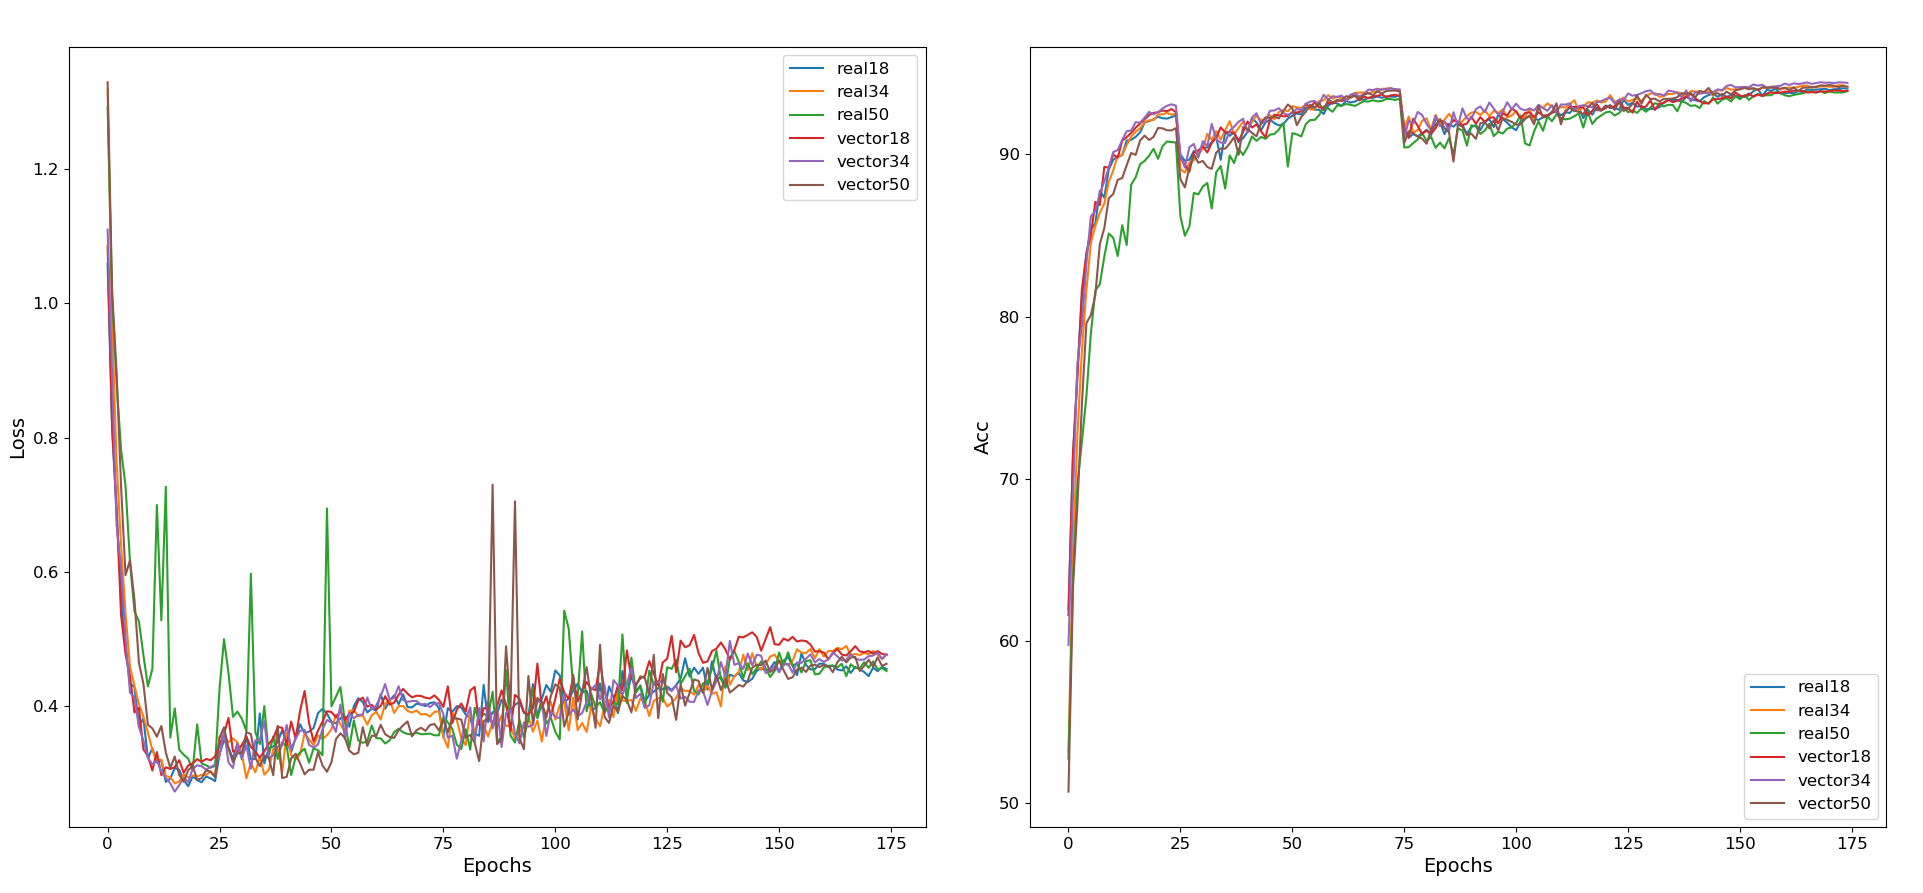
\includegraphics[width=1.0\columnwidth]{figures/loss.png}
		\caption{Validation loss and accuracy plots corresponding to the experimental runs that produced Table~\ref{t:results}.}
	\label{f:loss}
\end{figure}

\begin{figure}[h]
	\centering
		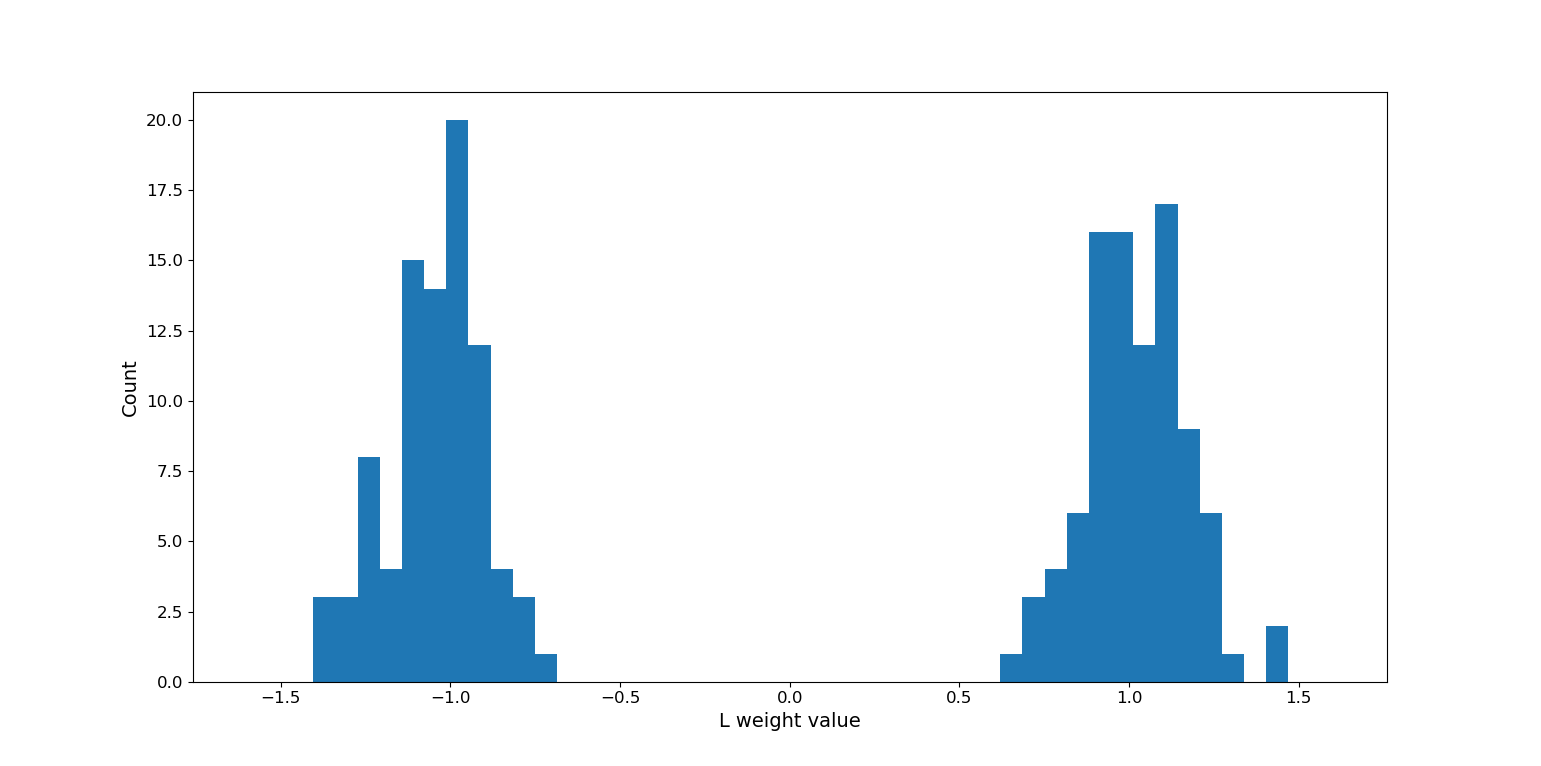
\includegraphics[width=1.0\columnwidth]{figures/hist.png}
		\caption{Histogram of $\textbf{L}$ values after training of the ResNet18 vector map convolution network.}
	\label{f:hist}
\end{figure}

\begin{figure}[h]
	\centering
		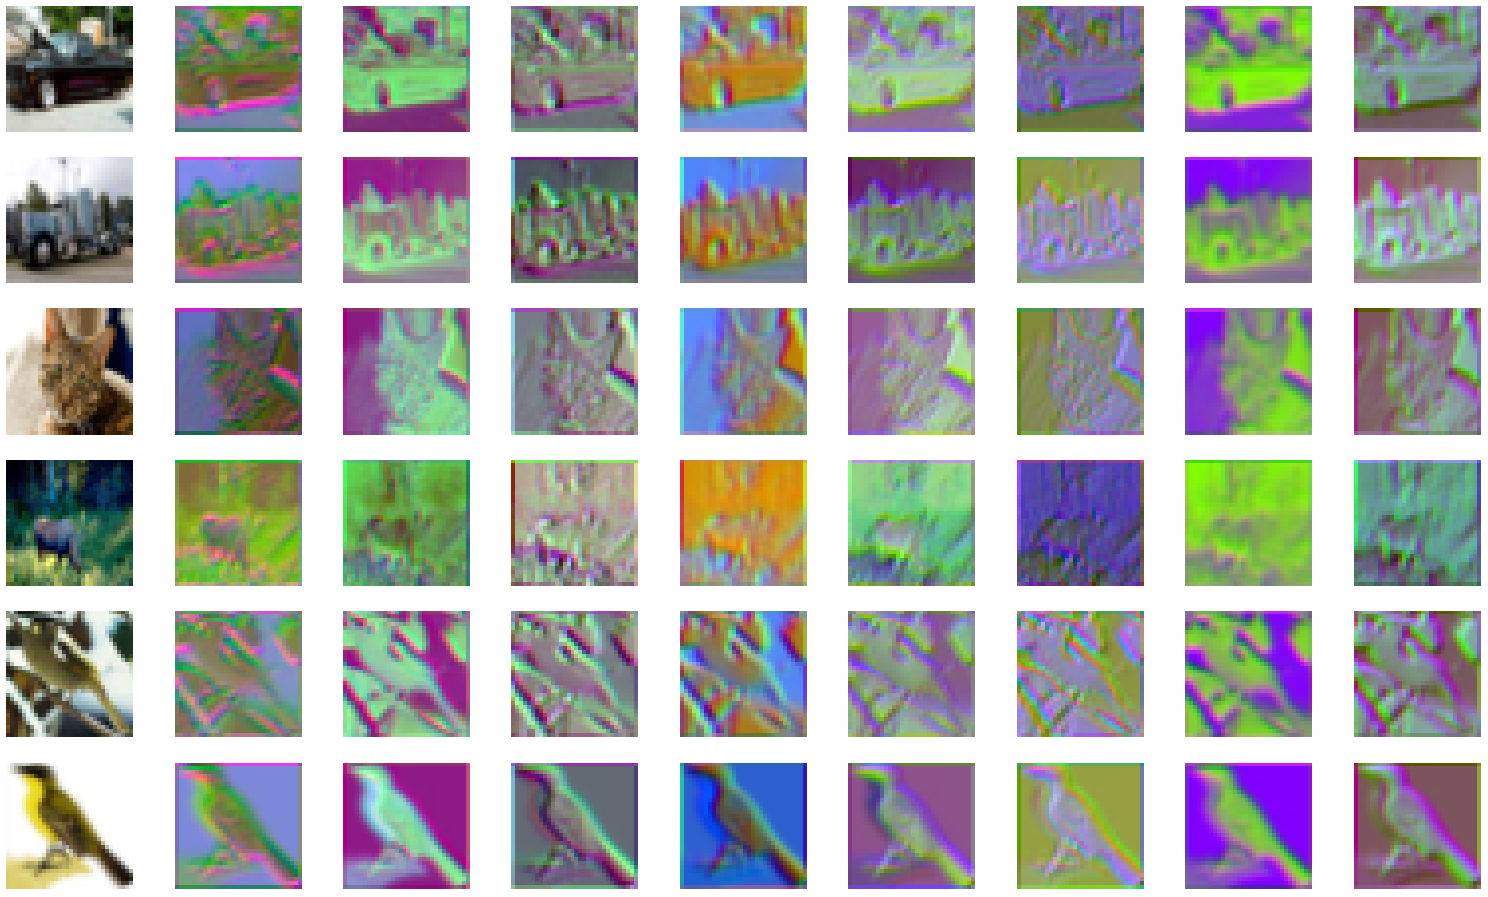
\includegraphics[width=1.0\columnwidth]{figures/samples.png}
		\caption{Randomly selected feature vector maps from the first convolution layer after training. Each row is a different image, where the first column are the original input images.}
	\label{f:samples}
\end{figure}


\section{Conclusions}
This paper proposes vector map convolutions to generalize the beneficial properties of convolutional complex and hyper-complex networks to any number of dimensions.
We also introduce a new learnable parameter to modify the linear combination of internal features.
The conducted experiments compare performance of vector map convolutions against real-valued networks in three different size ResNet models on CIFAR datasets.
They demonstrate that vector map convolution networks have similar accuracy at a reduced parameter count effectively mimicking hyper-complex networks.
We also investigate the distribution of the final values of $\textbf{L}$, the linear combination terms, and see that they also tend to stay around the value they were initialized to.
Future work will include comparison on data that is greater than five dimensions, like satellite images, against real-valued and hyper-complex networks.


\clearpage
%\bibliographystyle{plainnat}
\bibliographystyle{plain}
\bibliography{vMap}

\end{document}